\documentclass[1p]{elsarticle_modified}
%\bibliographystyle{elsarticle-num}

%\usepackage[colorlinks]{hyperref}
%\usepackage{abbrmath_seonhwa} %\Abb, \Ascr, \Acal ,\Abf, \Afrak
\usepackage{amsfonts}
\usepackage{amssymb}
\usepackage{amsmath}
\usepackage{amsthm}
\usepackage{scalefnt}
\usepackage{amsbsy}
\usepackage{kotex}
\usepackage{caption}
\usepackage{subfig}
\usepackage{color}
\usepackage{graphicx}
\usepackage{xcolor} %% white, black, red, green, blue, cyan, magenta, yellow
\usepackage{float}
\usepackage{setspace}
\usepackage{hyperref}

\usepackage{tikz}
\usetikzlibrary{arrows}

\usepackage{multirow}
\usepackage{array} % fixed length table
\usepackage{hhline}

%%%%%%%%%%%%%%%%%%%%%
\makeatletter
\renewcommand*\env@matrix[1][\arraystretch]{%
	\edef\arraystretch{#1}%
	\hskip -\arraycolsep
	\let\@ifnextchar\new@ifnextchar
	\array{*\c@MaxMatrixCols c}}
\makeatother %https://tex.stackexchange.com/questions/14071/how-can-i-increase-the-line-spacing-in-a-matrix
%%%%%%%%%%%%%%%

\usepackage[normalem]{ulem}

\newcommand{\msout}[1]{\ifmmode\text{\sout{\ensuremath{#1}}}\else\sout{#1}\fi}
%SOURCE: \msout is \stkout macro in https://tex.stackexchange.com/questions/20609/strikeout-in-math-mode

\newcommand{\cancel}[1]{
	\ifmmode
	{\color{red}\msout{#1}}
	\else
	{\color{red}\sout{#1}}
	\fi
}

\newcommand{\add}[1]{
	{\color{blue}\uwave{#1}}
}

\newcommand{\replace}[2]{
	\ifmmode
	{\color{red}\msout{#1}}{\color{blue}\uwave{#2}}
	\else
	{\color{red}\sout{#1}}{\color{blue}\uwave{#2}}
	\fi
}

\newcommand{\Sol}{\mathcal{S}} %segment
\newcommand{\D}{D} %diagram
\newcommand{\A}{\mathcal{A}} %arc


%%%%%%%%%%%%%%%%%%%%%%%%%%%%%5 test

\def\sl{\operatorname{\textup{SL}}(2,\Cbb)}
\def\psl{\operatorname{\textup{PSL}}(2,\Cbb)}
\def\quan{\mkern 1mu \triangleright \mkern 1mu}

\theoremstyle{definition}
\newtheorem{thm}{Theorem}[section]
\newtheorem{prop}[thm]{Proposition}
\newtheorem{lem}[thm]{Lemma}
\newtheorem{ques}[thm]{Question}
\newtheorem{cor}[thm]{Corollary}
\newtheorem{defn}[thm]{Definition}
\newtheorem{exam}[thm]{Example}
\newtheorem{rmk}[thm]{Remark}
\newtheorem{alg}[thm]{Algorithm}

\newcommand{\I}{\sqrt{-1}}
\begin{document}

%\begin{frontmatter}
%
%\title{Boundary parabolic representations of knots up to 8 crossings}
%
%%% Group authors per affiliation:
%\author{Yunhi Cho} 
%\address{Department of Mathematics, University of Seoul, Seoul, Korea}
%\ead{yhcho@uos.ac.kr}
%
%
%\author{Seonhwa Kim} %\fnref{s_kim}}
%\address{Center for Geometry and Physics, Institute for Basic Science, Pohang, 37673, Korea}
%\ead{ryeona17@ibs.re.kr}
%
%\author{Hyuk Kim}
%\address{Department of Mathematical Sciences, Seoul National University, Seoul 08826, Korea}
%\ead{hyukkim@snu.ac.kr}
%
%\author{Seokbeom Yoon}
%\address{Department of Mathematical Sciences, Seoul National University, Seoul, 08826,  Korea}
%\ead{sbyoon15@snu.ac.kr}
%
%\begin{abstract}
%We find all boundary parabolic representation of knots up to 8 crossings.
%
%\end{abstract}
%\begin{keyword}
%    \MSC[2010] 57M25 
%\end{keyword}
%
%\end{frontmatter}

%\linenumbers
%\tableofcontents
%
\newcommand\colored[1]{\textcolor{white}{\rule[-0.35ex]{0.8em}{1.4ex}}\kern-0.8em\color{red} #1}%
%\newcommand\colored[1]{\textcolor{white}{ #1}\kern-2.17ex	\textcolor{white}{ #1}\kern-1.81ex	\textcolor{white}{ #1}\kern-2.15ex\color{red}#1	}

{\Large $\underline{12a_{0395}~(K12a_{0395})}$}

\setlength{\tabcolsep}{10pt}
\renewcommand{\arraystretch}{1.6}
\vspace{1cm}\begin{tabular}{m{100pt}>{\centering\arraybackslash}m{274pt}}
\multirow{5}{120pt}{
	\centering
	\includegraphics[width=112pt]{../../../GIT/diagram.site/Diagrams/png/1196_12a_0395.png}\\
\ \ \ A knot diagram\footnotemark}&
\allowdisplaybreaks
\textbf{Linearized knot diagam} \\
\cline{2-2}
 &
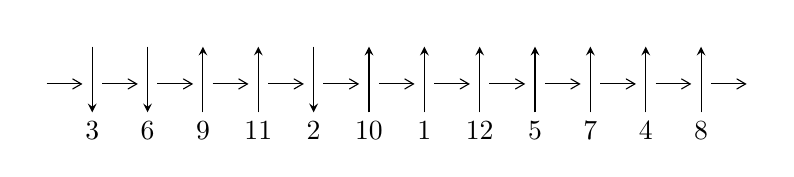
\begin{tikzpicture}[x=20pt, y=17pt]
	% nodes
	\node (C0) at (0, 0) {};
	\node (C1) at (1, 0) {};
	\node (C1U) at (1, +1) {};
	\node (C1D) at (1, -1) {3};

	\node (C2) at (2, 0) {};
	\node (C2U) at (2, +1) {};
	\node (C2D) at (2, -1) {6};

	\node (C3) at (3, 0) {};
	\node (C3U) at (3, +1) {};
	\node (C3D) at (3, -1) {9};

	\node (C4) at (4, 0) {};
	\node (C4U) at (4, +1) {};
	\node (C4D) at (4, -1) {11};

	\node (C5) at (5, 0) {};
	\node (C5U) at (5, +1) {};
	\node (C5D) at (5, -1) {2};

	\node (C6) at (6, 0) {};
	\node (C6U) at (6, +1) {};
	\node (C6D) at (6, -1) {10};

	\node (C7) at (7, 0) {};
	\node (C7U) at (7, +1) {};
	\node (C7D) at (7, -1) {1};

	\node (C8) at (8, 0) {};
	\node (C8U) at (8, +1) {};
	\node (C8D) at (8, -1) {12};

	\node (C9) at (9, 0) {};
	\node (C9U) at (9, +1) {};
	\node (C9D) at (9, -1) {5};

	\node (C10) at (10, 0) {};
	\node (C10U) at (10, +1) {};
	\node (C10D) at (10, -1) {7};

	\node (C11) at (11, 0) {};
	\node (C11U) at (11, +1) {};
	\node (C11D) at (11, -1) {4};

	\node (C12) at (12, 0) {};
	\node (C12U) at (12, +1) {};
	\node (C12D) at (12, -1) {8};
	\node (C13) at (13, 0) {};

	% arrows
	\draw[->,>={angle 60}]
	(C0) edge (C1) (C1) edge (C2) (C2) edge (C3) (C3) edge (C4) (C4) edge (C5) (C5) edge (C6) (C6) edge (C7) (C7) edge (C8) (C8) edge (C9) (C9) edge (C10) (C10) edge (C11) (C11) edge (C12) (C12) edge (C13) ;	\draw[->,>=stealth]
	(C1U) edge (C1D) (C2U) edge (C2D) (C3D) edge (C3U) (C4D) edge (C4U) (C5U) edge (C5D) (C6D) edge (C6U) (C7D) edge (C7U) (C8D) edge (C8U) (C9D) edge (C9U) (C10D) edge (C10U) (C11D) edge (C11U) (C12D) edge (C12U) ;
	\end{tikzpicture} \\
\hhline{~~} \\& 
\textbf{Solving Sequence} \\ \cline{2-2} 
 &
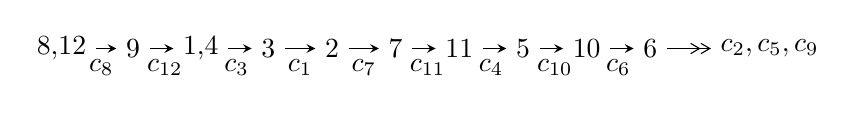
\begin{tikzpicture}[x=23pt, y=7pt]
	% node
	\node (A0) at (-1/8, 0) {8,12};
	\node (A1) at (1, 0) {9};
	\node (A2) at (33/16, 0) {1,4};
	\node (A3) at (25/8, 0) {3};
	\node (A4) at (33/8, 0) {2};
	\node (A5) at (41/8, 0) {7};
	\node (A6) at (49/8, 0) {11};
	\node (A7) at (57/8, 0) {5};
	\node (A8) at (65/8, 0) {10};
	\node (A9) at (73/8, 0) {6};
	\node (C1) at (1/2, -1) {$c_{8}$};
	\node (C2) at (3/2, -1) {$c_{12}$};
	\node (C3) at (21/8, -1) {$c_{3}$};
	\node (C4) at (29/8, -1) {$c_{1}$};
	\node (C5) at (37/8, -1) {$c_{7}$};
	\node (C6) at (45/8, -1) {$c_{11}$};
	\node (C7) at (53/8, -1) {$c_{4}$};
	\node (C8) at (61/8, -1) {$c_{10}$};
	\node (C9) at (69/8, -1) {$c_{6}$};
	\node (A10) at (11, 0) {$c_{2},c_{5},c_{9}$};

	% edge
	\draw[->,>=stealth]	
	(A0) edge (A1) (A1) edge (A2) (A2) edge (A3) (A3) edge (A4) (A4) edge (A5) (A5) edge (A6) (A6) edge (A7) (A7) edge (A8) (A8) edge (A9) ;
	\draw[->>,>={angle 60}]	
	(A9) edge (A10);
\end{tikzpicture} \\ 

\end{tabular} \\

\footnotetext{
The image of knot diagram is generated by the software ``\textbf{Draw programme}" developed by Andrew Bartholomew(\url{http://www.layer8.co.uk/maths/draw/index.htm\#Running-draw}), where we modified some parts for our purpose(\url{https://github.com/CATsTAILs/LinksPainter}).
}\phantom \\ \newline 
\centering \textbf{Ideals for irreducible components\footnotemark of $X_{\text{par}}$} 
 
\begin{align*}
I^u_{1}&=\langle 
2.65404\times10^{344} u^{118}-3.71960\times10^{344} u^{117}+\cdots+1.51948\times10^{345} b-8.39541\times10^{345},\\
\phantom{I^u_{1}}&\phantom{= \langle  }-4.85729\times10^{345} u^{118}-1.06056\times10^{346} u^{117}+\cdots+1.51948\times10^{345} a+4.54469\times10^{346},\\
\phantom{I^u_{1}}&\phantom{= \langle  }u^{119}+2 u^{118}+\cdots-26 u+1\rangle \\
I^u_{2}&=\langle 
- u^{27}+18 u^{26}+\cdots+b+13,\;-5 u^{26}+5 u^{25}+\cdots+a-5,\;u^{28}- u^{27}+\cdots+6 u^2+1\rangle \\
\\
\end{align*}
\raggedright * 2 irreducible components of $\dim_{\mathbb{C}}=0$, with total 147 representations.\\
\footnotetext{All coefficients of polynomials are rational numbers. But the coefficients are sometimes approximated in decimal forms when there is not enough margin.}
\newpage
\renewcommand{\arraystretch}{1}
\centering \section*{I. $I^u_{1}= \langle 2.65\times10^{344} u^{118}-3.72\times10^{344} u^{117}+\cdots+1.52\times10^{345} b-8.40\times10^{345},\;-4.86\times10^{345} u^{118}-1.06\times10^{346} u^{117}+\cdots+1.52\times10^{345} a+4.54\times10^{346},\;u^{119}+2 u^{118}+\cdots-26 u+1 \rangle$}
\flushleft \textbf{(i) Arc colorings}\\
\begin{tabular}{m{7pt} m{180pt} m{7pt} m{180pt} }
\flushright $a_{8}=$&$\begin{pmatrix}1\\0\end{pmatrix}$ \\
\flushright $a_{12}=$&$\begin{pmatrix}0\\u\end{pmatrix}$ \\
\flushright $a_{9}=$&$\begin{pmatrix}1\\- u^2\end{pmatrix}$ \\
\flushright $a_{1}=$&$\begin{pmatrix}u\\u\end{pmatrix}$ \\
\flushright $a_{4}=$&$\begin{pmatrix}3.19669 u^{118}+6.97979 u^{117}+\cdots+513.032 u-29.9096\\-0.174668 u^{118}+0.244795 u^{117}+\cdots-62.1195 u+5.52519\end{pmatrix}$ \\
\flushright $a_{3}=$&$\begin{pmatrix}3.45928 u^{118}+7.64632 u^{117}+\cdots+563.101 u-34.8483\\-0.208279 u^{118}+0.424943 u^{117}+\cdots-65.5319 u+5.66654\end{pmatrix}$ \\
\flushright $a_{2}=$&$\begin{pmatrix}-1.55048 u^{118}-3.05586 u^{117}+\cdots-520.403 u+40.2446\\0.373680 u^{118}+0.462149 u^{117}+\cdots-61.8390 u+3.46753\end{pmatrix}$ \\
\flushright $a_{7}=$&$\begin{pmatrix}u^2+1\\u^2\end{pmatrix}$ \\
\flushright $a_{11}=$&$\begin{pmatrix}-3.38646 u^{118}-6.55223 u^{117}+\cdots-668.355 u+47.2932\\-0.293160 u^{118}+0.510861 u^{117}+\cdots-51.3704 u+2.09553\end{pmatrix}$ \\
\flushright $a_{5}=$&$\begin{pmatrix}1.68383 u^{118}+3.07028 u^{117}+\cdots+512.719 u-38.2522\\-0.497398 u^{118}-1.60028 u^{117}+\cdots+16.7133 u-0.0504918\end{pmatrix}$ \\
\flushright $a_{10}=$&$\begin{pmatrix}-3.52942 u^{118}-7.11188 u^{117}+\cdots-628.685 u+45.7434\\-1.04054 u^{118}-1.58837 u^{117}+\cdots-43.3753 u+1.76478\end{pmatrix}$ \\
\flushright $a_{6}=$&$\begin{pmatrix}1.84545 u^{118}+3.19677 u^{117}+\cdots+336.654 u-40.3459\\0.339358 u^{118}-0.259898 u^{117}+\cdots+120.671 u-6.71138\end{pmatrix}$\\&\end{tabular}
\flushleft \textbf{(ii) Obstruction class $= -1$}\\~\\
\flushleft \textbf{(iii) Cusp Shapes $= -2.64123 u^{118}-5.23612 u^{117}+\cdots-267.516 u+30.7025$}\\~\\
\newpage\renewcommand{\arraystretch}{1}
\flushleft \textbf{(iv) u-Polynomials at the component}\newline \\
\begin{tabular}{m{50pt}|m{274pt}}
Crossings & \hspace{64pt}u-Polynomials at each crossing \\
\hline $$\begin{aligned}c_{1}\end{aligned}$$&$\begin{aligned}
&u^{119}+51 u^{118}+\cdots+26772 u+361
\end{aligned}$\\
\hline $$\begin{aligned}c_{2},c_{5}\end{aligned}$$&$\begin{aligned}
&u^{119}+7 u^{118}+\cdots-208 u-19
\end{aligned}$\\
\hline $$\begin{aligned}c_{3}\end{aligned}$$&$\begin{aligned}
&u^{119}- u^{118}+\cdots-25185412 u-11522837
\end{aligned}$\\
\hline $$\begin{aligned}c_{4},c_{11}\end{aligned}$$&$\begin{aligned}
&u^{119}-3 u^{118}+\cdots-2732 u-8803
\end{aligned}$\\
\hline $$\begin{aligned}c_{6},c_{10}\end{aligned}$$&$\begin{aligned}
&u^{119}+3 u^{118}+\cdots-4107 u-2939
\end{aligned}$\\
\hline $$\begin{aligned}c_{7},c_{8},c_{12}\end{aligned}$$&$\begin{aligned}
&u^{119}-2 u^{118}+\cdots-26 u-1
\end{aligned}$\\
\hline $$\begin{aligned}c_{9}\end{aligned}$$&$\begin{aligned}
&u^{119}+u^{118}+\cdots+8910 u-1089
\end{aligned}$\\
\hline
\end{tabular}\\~\\
\newpage\renewcommand{\arraystretch}{1}
\flushleft \textbf{(v) Riley Polynomials at the component}\newline \\
\begin{tabular}{m{50pt}|m{274pt}}
Crossings & \hspace{64pt}Riley Polynomials at each crossing \\
\hline $$\begin{aligned}c_{1}\end{aligned}$$&$\begin{aligned}
&y^{119}+49 y^{118}+\cdots+68785416 y-130321
\end{aligned}$\\
\hline $$\begin{aligned}c_{2},c_{5}\end{aligned}$$&$\begin{aligned}
&y^{119}-51 y^{118}+\cdots+26772 y-361
\end{aligned}$\\
\hline $$\begin{aligned}c_{3}\end{aligned}$$&$\begin{aligned}
&y^{119}+43 y^{118}+\cdots-5505345069862148 y-132775772528569
\end{aligned}$\\
\hline $$\begin{aligned}c_{4},c_{11}\end{aligned}$$&$\begin{aligned}
&y^{119}+95 y^{118}+\cdots-90407930 y-77492809
\end{aligned}$\\
\hline $$\begin{aligned}c_{6},c_{10}\end{aligned}$$&$\begin{aligned}
&y^{119}-75 y^{118}+\cdots+495977351 y-8637721
\end{aligned}$\\
\hline $$\begin{aligned}c_{7},c_{8},c_{12}\end{aligned}$$&$\begin{aligned}
&y^{119}+120 y^{118}+\cdots+210 y-1
\end{aligned}$\\
\hline $$\begin{aligned}c_{9}\end{aligned}$$&$\begin{aligned}
&y^{119}-13 y^{118}+\cdots-26164314 y-1185921
\end{aligned}$\\
\hline
\end{tabular}\\~\\
\newpage\flushleft \textbf{(vi) Complex Volumes and Cusp Shapes}
$$\begin{array}{c|c|c}  
\text{Solutions to }I^u_{1}& \I (\text{vol} + \sqrt{-1}CS) & \text{Cusp shape}\\
 \hline 
\begin{aligned}
u &= \phantom{-}0.355122 + 0.928118 I \\
a &= \phantom{-}0.550756 - 0.398938 I \\
b &= \phantom{-}1.14338 - 0.84841 I\end{aligned}
 & \phantom{-}3.73858 + 1.09865 I & \phantom{-0.000000 } 0 \\ \hline\begin{aligned}
u &= \phantom{-}0.355122 - 0.928118 I \\
a &= \phantom{-}0.550756 + 0.398938 I \\
b &= \phantom{-}1.14338 + 0.84841 I\end{aligned}
 & \phantom{-}3.73858 - 1.09865 I & \phantom{-0.000000 } 0 \\ \hline\begin{aligned}
u &= \phantom{-}0.437780 + 0.889964 I \\
a &= -0.413334 + 0.259923 I \\
b &= -1.15550 + 0.89782 I\end{aligned}
 & \phantom{-}2.52193 - 4.36091 I & \phantom{-0.000000 } 0 \\ \hline\begin{aligned}
u &= \phantom{-}0.437780 - 0.889964 I \\
a &= -0.413334 - 0.259923 I \\
b &= -1.15550 - 0.89782 I\end{aligned}
 & \phantom{-}2.52193 + 4.36091 I & \phantom{-0.000000 } 0 \\ \hline\begin{aligned}
u &= -0.845759 + 0.501522 I \\
a &= \phantom{-}1.092950 - 0.875220 I \\
b &= \phantom{-}0.953716 + 0.274130 I\end{aligned}
 & \phantom{-}1.93927 - 7.77593 I & \phantom{-0.000000 } 0 \\ \hline\begin{aligned}
u &= -0.845759 - 0.501522 I \\
a &= \phantom{-}1.092950 + 0.875220 I \\
b &= \phantom{-}0.953716 - 0.274130 I\end{aligned}
 & \phantom{-}1.93927 + 7.77593 I & \phantom{-0.000000 } 0 \\ \hline\begin{aligned}
u &= \phantom{-}0.875445 + 0.381861 I \\
a &= \phantom{-}0.405474 + 1.234410 I \\
b &= \phantom{-}0.313119 - 0.353758 I\end{aligned}
 & -2.76497 - 2.55600 I & \phantom{-0.000000 } 0 \\ \hline\begin{aligned}
u &= \phantom{-}0.875445 - 0.381861 I \\
a &= \phantom{-}0.405474 - 1.234410 I \\
b &= \phantom{-}0.313119 + 0.353758 I\end{aligned}
 & -2.76497 + 2.55600 I & \phantom{-0.000000 } 0 \\ \hline\begin{aligned}
u &= -0.705215 + 0.782711 I \\
a &= -1.117440 + 0.448086 I \\
b &= -1.055030 - 0.080011 I\end{aligned}
 & -4.11674 - 5.83144 I & \phantom{-0.000000 } 0 \\ \hline\begin{aligned}
u &= -0.705215 - 0.782711 I \\
a &= -1.117440 - 0.448086 I \\
b &= -1.055030 + 0.080011 I\end{aligned}
 & -4.11674 + 5.83144 I & \phantom{-0.000000 } 0\\
 \hline 
 \end{array}$$\newpage$$\begin{array}{c|c|c}  
\text{Solutions to }I^u_{1}& \I (\text{vol} + \sqrt{-1}CS) & \text{Cusp shape}\\
 \hline 
\begin{aligned}
u &= -0.757241 + 0.738794 I \\
a &= \phantom{-}0.530380 - 0.966180 I \\
b &= \phantom{-}0.964868 - 0.113031 I\end{aligned}
 & \phantom{-}1.31392 + 2.27943 I & \phantom{-0.000000 } 0 \\ \hline\begin{aligned}
u &= -0.757241 - 0.738794 I \\
a &= \phantom{-}0.530380 + 0.966180 I \\
b &= \phantom{-}0.964868 + 0.113031 I\end{aligned}
 & \phantom{-}1.31392 - 2.27943 I & \phantom{-0.000000 } 0 \\ \hline\begin{aligned}
u &= -0.951437 + 0.538602 I \\
a &= -0.954025 + 0.834561 I \\
b &= -1.006380 - 0.310638 I\end{aligned}
 & \phantom{-}0.09823 - 13.43470 I & \phantom{-0.000000 } 0 \\ \hline\begin{aligned}
u &= -0.951437 - 0.538602 I \\
a &= -0.954025 - 0.834561 I \\
b &= -1.006380 + 0.310638 I\end{aligned}
 & \phantom{-}0.09823 + 13.43470 I & \phantom{-0.000000 } 0 \\ \hline\begin{aligned}
u &= \phantom{-}0.695269 + 0.547167 I \\
a &= \phantom{-}1.12801 + 0.86039 I \\
b &= \phantom{-}1.313030 + 0.247781 I\end{aligned}
 & -3.35283 + 7.39480 I & \phantom{-0.000000 } 0 \\ \hline\begin{aligned}
u &= \phantom{-}0.695269 - 0.547167 I \\
a &= \phantom{-}1.12801 - 0.86039 I \\
b &= \phantom{-}1.313030 - 0.247781 I\end{aligned}
 & -3.35283 - 7.39480 I & \phantom{-0.000000 } 0 \\ \hline\begin{aligned}
u &= \phantom{-}1.112250 + 0.084793 I \\
a &= \phantom{-}0.065711 + 1.222590 I \\
b &= \phantom{-}0.053847 - 0.423809 I\end{aligned}
 & -3.19379 + 1.91472 I & \phantom{-0.000000 } 0 \\ \hline\begin{aligned}
u &= \phantom{-}1.112250 - 0.084793 I \\
a &= \phantom{-}0.065711 - 1.222590 I \\
b &= \phantom{-}0.053847 + 0.423809 I\end{aligned}
 & -3.19379 - 1.91472 I & \phantom{-0.000000 } 0 \\ \hline\begin{aligned}
u &= -1.081990 + 0.417768 I \\
a &= -0.237717 + 0.919197 I \\
b &= -0.527929 - 0.155026 I\end{aligned}
 & -2.65576 - 0.04297 I & \phantom{-0.000000 } 0 \\ \hline\begin{aligned}
u &= -1.081990 - 0.417768 I \\
a &= -0.237717 - 0.919197 I \\
b &= -0.527929 + 0.155026 I\end{aligned}
 & -2.65576 + 0.04297 I & \phantom{-0.000000 } 0\\
 \hline 
 \end{array}$$\newpage$$\begin{array}{c|c|c}  
\text{Solutions to }I^u_{1}& \I (\text{vol} + \sqrt{-1}CS) & \text{Cusp shape}\\
 \hline 
\begin{aligned}
u &= \phantom{-}0.641878 + 0.455011 I \\
a &= -1.12839 - 1.00439 I \\
b &= -1.134130 - 0.121220 I\end{aligned}
 & -1.97592 + 2.57078 I & \phantom{-0.000000 } 0 \\ \hline\begin{aligned}
u &= \phantom{-}0.641878 - 0.455011 I \\
a &= -1.12839 + 1.00439 I \\
b &= -1.134130 + 0.121220 I\end{aligned}
 & -1.97592 - 2.57078 I & \phantom{-0.000000 } 0 \\ \hline\begin{aligned}
u &= \phantom{-}0.675053 + 0.328204 I \\
a &= \phantom{-}1.136430 - 0.608303 I \\
b &= \phantom{-}0.237290 + 0.356326 I\end{aligned}
 & \phantom{-}4.09882 + 8.36988 I & \phantom{-0.000000 } 0 \\ \hline\begin{aligned}
u &= \phantom{-}0.675053 - 0.328204 I \\
a &= \phantom{-}1.136430 + 0.608303 I \\
b &= \phantom{-}0.237290 - 0.356326 I\end{aligned}
 & \phantom{-}4.09882 - 8.36988 I & \phantom{-0.000000 } 0 \\ \hline\begin{aligned}
u &= \phantom{-}0.634326 + 0.392829 I \\
a &= -0.81207 - 1.22851 I \\
b &= -0.611921 + 0.198271 I\end{aligned}
 & -1.91605 + 1.49481 I & \phantom{-0.000000 } 0 \\ \hline\begin{aligned}
u &= \phantom{-}0.634326 - 0.392829 I \\
a &= -0.81207 + 1.22851 I \\
b &= -0.611921 - 0.198271 I\end{aligned}
 & -1.91605 - 1.49481 I & \phantom{-0.000000 } 0 \\ \hline\begin{aligned}
u &= -0.240172 + 1.238760 I \\
a &= -0.556332 + 0.086031 I \\
b &= -0.113358 + 1.141540 I\end{aligned}
 & -0.726114 - 0.980196 I & \phantom{-0.000000 } 0 \\ \hline\begin{aligned}
u &= -0.240172 - 1.238760 I \\
a &= -0.556332 - 0.086031 I \\
b &= -0.113358 - 1.141540 I\end{aligned}
 & -0.726114 + 0.980196 I & \phantom{-0.000000 } 0 \\ \hline\begin{aligned}
u &= -0.484304 + 0.554618 I \\
a &= -0.606336 - 0.560699 I \\
b &= -0.616895 + 0.079272 I\end{aligned}
 & \phantom{-}0.41624 - 4.00939 I & \phantom{-0.000000 } 0 \\ \hline\begin{aligned}
u &= -0.484304 - 0.554618 I \\
a &= -0.606336 + 0.560699 I \\
b &= -0.616895 - 0.079272 I\end{aligned}
 & \phantom{-}0.41624 + 4.00939 I & \phantom{-0.000000 } 0\\
 \hline 
 \end{array}$$\newpage$$\begin{array}{c|c|c}  
\text{Solutions to }I^u_{1}& \I (\text{vol} + \sqrt{-1}CS) & \text{Cusp shape}\\
 \hline 
\begin{aligned}
u &= -0.264408 + 1.242480 I \\
a &= \phantom{-}0.477396 - 0.193983 I \\
b &= -0.348744 - 0.889733 I\end{aligned}
 & -1.11104 - 6.19546 I & \phantom{-0.000000 } 0 \\ \hline\begin{aligned}
u &= -0.264408 - 1.242480 I \\
a &= \phantom{-}0.477396 + 0.193983 I \\
b &= -0.348744 + 0.889733 I\end{aligned}
 & -1.11104 + 6.19546 I & \phantom{-0.000000 } 0 \\ \hline\begin{aligned}
u &= -0.964873 + 0.827467 I \\
a &= -0.468445 + 0.848498 I \\
b &= -0.992484 - 0.116628 I\end{aligned}
 & -0.55827 + 7.05368 I & \phantom{-0.000000 } 0 \\ \hline\begin{aligned}
u &= -0.964873 - 0.827467 I \\
a &= -0.468445 - 0.848498 I \\
b &= -0.992484 + 0.116628 I\end{aligned}
 & -0.55827 - 7.05368 I & \phantom{-0.000000 } 0 \\ \hline\begin{aligned}
u &= \phantom{-}0.095017 + 1.278750 I \\
a &= -0.650456 - 0.592085 I \\
b &= -0.693055 + 0.490549 I\end{aligned}
 & -1.97975 - 4.57227 I & \phantom{-0.000000 } 0 \\ \hline\begin{aligned}
u &= \phantom{-}0.095017 - 1.278750 I \\
a &= -0.650456 + 0.592085 I \\
b &= -0.693055 - 0.490549 I\end{aligned}
 & -1.97975 + 4.57227 I & \phantom{-0.000000 } 0 \\ \hline\begin{aligned}
u &= -0.225905 + 1.265030 I \\
a &= -0.537859 - 0.450634 I \\
b &= -0.724965 + 0.412460 I\end{aligned}
 & -1.26041 - 0.68479 I & \phantom{-0.000000 } 0 \\ \hline\begin{aligned}
u &= -0.225905 - 1.265030 I \\
a &= -0.537859 + 0.450634 I \\
b &= -0.724965 - 0.412460 I\end{aligned}
 & -1.26041 + 0.68479 I & \phantom{-0.000000 } 0 \\ \hline\begin{aligned}
u &= -0.699562 + 0.012160 I \\
a &= \phantom{-}0.572503 - 0.802595 I \\
b &= \phantom{-}0.331384 - 0.700904 I\end{aligned}
 & \phantom{-}2.66598 + 2.68142 I & \phantom{-0.000000 } 0 \\ \hline\begin{aligned}
u &= -0.699562 - 0.012160 I \\
a &= \phantom{-}0.572503 + 0.802595 I \\
b &= \phantom{-}0.331384 + 0.700904 I\end{aligned}
 & \phantom{-}2.66598 - 2.68142 I & \phantom{-0.000000 } 0\\
 \hline 
 \end{array}$$\newpage$$\begin{array}{c|c|c}  
\text{Solutions to }I^u_{1}& \I (\text{vol} + \sqrt{-1}CS) & \text{Cusp shape}\\
 \hline 
\begin{aligned}
u &= \phantom{-}0.453308 + 0.523255 I \\
a &= -1.017620 - 0.478761 I \\
b &= -0.985184 + 0.688651 I\end{aligned}
 & -1.41515 + 1.44928 I & \phantom{-0.000000 } 0 \\ \hline\begin{aligned}
u &= \phantom{-}0.453308 - 0.523255 I \\
a &= -1.017620 + 0.478761 I \\
b &= -0.985184 - 0.688651 I\end{aligned}
 & -1.41515 - 1.44928 I & \phantom{-0.000000 } 0 \\ \hline\begin{aligned}
u &= \phantom{-}0.428626 + 0.530864 I \\
a &= \phantom{-}1.64427 + 0.93701 I \\
b &= \phantom{-}0.865572 + 0.646236 I\end{aligned}
 & -6.41806 + 1.42312 I & \phantom{-0.000000 } 0 \\ \hline\begin{aligned}
u &= \phantom{-}0.428626 - 0.530864 I \\
a &= \phantom{-}1.64427 - 0.93701 I \\
b &= \phantom{-}0.865572 - 0.646236 I\end{aligned}
 & -6.41806 - 1.42312 I & \phantom{-0.000000 } 0 \\ \hline\begin{aligned}
u &= -0.305414 + 0.597967 I \\
a &= \phantom{-}0.95867 - 1.19353 I \\
b &= \phantom{-}1.014210 - 0.576340 I\end{aligned}
 & \phantom{-}1.23996 + 1.80948 I & \phantom{-}6.00000 + 0. I\phantom{ +0.000000I} \\ \hline\begin{aligned}
u &= -0.305414 - 0.597967 I \\
a &= \phantom{-}0.95867 + 1.19353 I \\
b &= \phantom{-}1.014210 + 0.576340 I\end{aligned}
 & \phantom{-}1.23996 - 1.80948 I & \phantom{-}6.00000 + 0. I\phantom{ +0.000000I} \\ \hline\begin{aligned}
u &= \phantom{-}0.623047 + 0.229109 I \\
a &= -1.41218 + 0.62072 I \\
b &= -0.188966 - 0.236767 I\end{aligned}
 & \phantom{-}5.77681 + 2.48293 I & \phantom{-}12.94457 - 3.64631 I \\ \hline\begin{aligned}
u &= \phantom{-}0.623047 - 0.229109 I \\
a &= -1.41218 - 0.62072 I \\
b &= -0.188966 + 0.236767 I\end{aligned}
 & \phantom{-}5.77681 - 2.48293 I & \phantom{-}12.94457 + 3.64631 I \\ \hline\begin{aligned}
u &= -0.565817 + 0.318993 I \\
a &= \phantom{-}0.626424 + 0.495344 I \\
b &= \phantom{-}0.530615 + 0.076115 I\end{aligned}
 & \phantom{-}1.123500 + 0.392328 I & \phantom{-}10.23388 + 0. I\phantom{ +0.000000I} \\ \hline\begin{aligned}
u &= -0.565817 - 0.318993 I \\
a &= \phantom{-}0.626424 - 0.495344 I \\
b &= \phantom{-}0.530615 - 0.076115 I\end{aligned}
 & \phantom{-}1.123500 - 0.392328 I & \phantom{-}10.23388 + 0. I\phantom{ +0.000000I}\\
 \hline 
 \end{array}$$\newpage$$\begin{array}{c|c|c}  
\text{Solutions to }I^u_{1}& \I (\text{vol} + \sqrt{-1}CS) & \text{Cusp shape}\\
 \hline 
\begin{aligned}
u &= -0.230407 + 1.346620 I \\
a &= \phantom{-}0.081429 - 0.280356 I \\
b &= -0.329335 - 0.132775 I\end{aligned}
 & -3.97108 - 2.43584 I & \phantom{-0.000000 } 0 \\ \hline\begin{aligned}
u &= -0.230407 - 1.346620 I \\
a &= \phantom{-}0.081429 + 0.280356 I \\
b &= -0.329335 + 0.132775 I\end{aligned}
 & -3.97108 + 2.43584 I & \phantom{-0.000000 } 0 \\ \hline\begin{aligned}
u &= -0.071954 + 1.381730 I \\
a &= -0.149743 - 0.485375 I \\
b &= -0.590332 - 0.059182 I\end{aligned}
 & -3.85572 - 1.71095 I & \phantom{-0.000000 } 0 \\ \hline\begin{aligned}
u &= -0.071954 - 1.381730 I \\
a &= -0.149743 + 0.485375 I \\
b &= -0.590332 + 0.059182 I\end{aligned}
 & -3.85572 + 1.71095 I & \phantom{-0.000000 } 0 \\ \hline\begin{aligned}
u &= -0.185869 + 1.371190 I \\
a &= \phantom{-}0.560257 + 0.491962 I \\
b &= \phantom{-}0.755665 - 0.451477 I\end{aligned}
 & -1.51610 - 4.94231 I & \phantom{-0.000000 } 0 \\ \hline\begin{aligned}
u &= -0.185869 - 1.371190 I \\
a &= \phantom{-}0.560257 - 0.491962 I \\
b &= \phantom{-}0.755665 + 0.451477 I\end{aligned}
 & -1.51610 + 4.94231 I & \phantom{-0.000000 } 0 \\ \hline\begin{aligned}
u &= \phantom{-}0.022030 + 1.384840 I \\
a &= \phantom{-}1.283010 - 0.173050 I \\
b &= \phantom{-}3.44123 + 0.33674 I\end{aligned}
 & -5.42143 + 3.44426 I & \phantom{-0.000000 } 0 \\ \hline\begin{aligned}
u &= \phantom{-}0.022030 - 1.384840 I \\
a &= \phantom{-}1.283010 + 0.173050 I \\
b &= \phantom{-}3.44123 - 0.33674 I\end{aligned}
 & -5.42143 - 3.44426 I & \phantom{-0.000000 } 0 \\ \hline\begin{aligned}
u &= -0.611413 + 0.036672 I \\
a &= -0.625202 + 1.115140 I \\
b &= -0.071919 + 0.898469 I\end{aligned}
 & \phantom{-}2.99131 - 2.19855 I & \phantom{-}11.46185 + 4.70957 I \\ \hline\begin{aligned}
u &= -0.611413 - 0.036672 I \\
a &= -0.625202 - 1.115140 I \\
b &= -0.071919 - 0.898469 I\end{aligned}
 & \phantom{-}2.99131 + 2.19855 I & \phantom{-}11.46185 - 4.70957 I\\
 \hline 
 \end{array}$$\newpage$$\begin{array}{c|c|c}  
\text{Solutions to }I^u_{1}& \I (\text{vol} + \sqrt{-1}CS) & \text{Cusp shape}\\
 \hline 
\begin{aligned}
u &= \phantom{-}0.009442 + 1.389940 I \\
a &= \phantom{-}0.597050 + 0.553267 I \\
b &= \phantom{-}0.726809 - 0.497772 I\end{aligned}
 & -1.90973 - 0.74900 I & \phantom{-0.000000 } 0 \\ \hline\begin{aligned}
u &= \phantom{-}0.009442 - 1.389940 I \\
a &= \phantom{-}0.597050 - 0.553267 I \\
b &= \phantom{-}0.726809 + 0.497772 I\end{aligned}
 & -1.90973 + 0.74900 I & \phantom{-0.000000 } 0 \\ \hline\begin{aligned}
u &= \phantom{-}0.068252 + 1.395030 I \\
a &= \phantom{-}0.799590 - 0.024691 I \\
b &= \phantom{-}4.16098 - 0.65705 I\end{aligned}
 & -2.63776 + 7.11139 I & \phantom{-0.000000 } 0 \\ \hline\begin{aligned}
u &= \phantom{-}0.068252 - 1.395030 I \\
a &= \phantom{-}0.799590 + 0.024691 I \\
b &= \phantom{-}4.16098 + 0.65705 I\end{aligned}
 & -2.63776 - 7.11139 I & \phantom{-0.000000 } 0 \\ \hline\begin{aligned}
u &= \phantom{-}0.019788 + 1.405330 I \\
a &= -0.787884 + 0.025430 I \\
b &= -3.83254 + 1.05902 I\end{aligned}
 & -2.12066 + 1.34209 I & \phantom{-0.000000 } 0 \\ \hline\begin{aligned}
u &= \phantom{-}0.019788 - 1.405330 I \\
a &= -0.787884 - 0.025430 I \\
b &= -3.83254 - 1.05902 I\end{aligned}
 & -2.12066 - 1.34209 I & \phantom{-0.000000 } 0 \\ \hline\begin{aligned}
u &= \phantom{-}0.178838 + 1.397610 I \\
a &= \phantom{-}0.280190 - 0.972222 I \\
b &= \phantom{-}0.514942 - 1.214260 I\end{aligned}
 & \phantom{-}0.59675 + 5.29093 I & \phantom{-0.000000 } 0 \\ \hline\begin{aligned}
u &= \phantom{-}0.178838 - 1.397610 I \\
a &= \phantom{-}0.280190 + 0.972222 I \\
b &= \phantom{-}0.514942 + 1.214260 I\end{aligned}
 & \phantom{-}0.59675 - 5.29093 I & \phantom{-0.000000 } 0 \\ \hline\begin{aligned}
u &= -0.02863 + 1.43149 I \\
a &= -1.263290 + 0.492520 I \\
b &= -3.09033 + 0.24494 I\end{aligned}
 & -6.34108 - 3.66733 I & \phantom{-0.000000 } 0 \\ \hline\begin{aligned}
u &= -0.02863 - 1.43149 I \\
a &= -1.263290 - 0.492520 I \\
b &= -3.09033 - 0.24494 I\end{aligned}
 & -6.34108 + 3.66733 I & \phantom{-0.000000 } 0\\
 \hline 
 \end{array}$$\newpage$$\begin{array}{c|c|c}  
\text{Solutions to }I^u_{1}& \I (\text{vol} + \sqrt{-1}CS) & \text{Cusp shape}\\
 \hline 
\begin{aligned}
u &= \phantom{-}0.22631 + 1.45071 I \\
a &= -0.223160 + 0.875930 I \\
b &= -0.421321 + 0.944082 I\end{aligned}
 & -1.66872 + 11.59560 I & \phantom{-0.000000 } 0 \\ \hline\begin{aligned}
u &= \phantom{-}0.22631 - 1.45071 I \\
a &= -0.223160 - 0.875930 I \\
b &= -0.421321 - 0.944082 I\end{aligned}
 & -1.66872 - 11.59560 I & \phantom{-0.000000 } 0 \\ \hline\begin{aligned}
u &= \phantom{-}0.41059 + 1.41053 I \\
a &= \phantom{-}0.976432 + 0.144840 I \\
b &= \phantom{-}2.63906 + 0.49267 I\end{aligned}
 & -7.57844 + 3.50049 I & \phantom{-0.000000 } 0 \\ \hline\begin{aligned}
u &= \phantom{-}0.41059 - 1.41053 I \\
a &= \phantom{-}0.976432 - 0.144840 I \\
b &= \phantom{-}2.63906 - 0.49267 I\end{aligned}
 & -7.57844 - 3.50049 I & \phantom{-0.000000 } 0 \\ \hline\begin{aligned}
u &= -0.334922 + 0.409655 I \\
a &= \phantom{-}2.57491 - 0.45039 I \\
b &= \phantom{-}0.640329 + 0.086594 I\end{aligned}
 & \phantom{-}1.54320 - 3.79998 I & \phantom{-}8.38218 + 10.90850 I \\ \hline\begin{aligned}
u &= -0.334922 - 0.409655 I \\
a &= \phantom{-}2.57491 + 0.45039 I \\
b &= \phantom{-}0.640329 - 0.086594 I\end{aligned}
 & \phantom{-}1.54320 + 3.79998 I & \phantom{-}8.38218 - 10.90850 I \\ \hline\begin{aligned}
u &= \phantom{-}0.234996 + 0.472015 I \\
a &= -0.34460 - 1.75071 I \\
b &= -0.324245 + 0.319005 I\end{aligned}
 & -1.57985 + 1.04137 I & -2.49531 - 4.65112 I \\ \hline\begin{aligned}
u &= \phantom{-}0.234996 - 0.472015 I \\
a &= -0.34460 + 1.75071 I \\
b &= -0.324245 - 0.319005 I\end{aligned}
 & -1.57985 - 1.04137 I & -2.49531 + 4.65112 I \\ \hline\begin{aligned}
u &= \phantom{-}0.05301 + 1.48085 I \\
a &= \phantom{-}0.200024 + 0.748713 I \\
b &= \phantom{-}0.770060 + 0.614245 I\end{aligned}
 & -7.97482 + 1.97792 I & \phantom{-0.000000 } 0 \\ \hline\begin{aligned}
u &= \phantom{-}0.05301 - 1.48085 I \\
a &= \phantom{-}0.200024 - 0.748713 I \\
b &= \phantom{-}0.770060 - 0.614245 I\end{aligned}
 & -7.97482 - 1.97792 I & \phantom{-0.000000 } 0\\
 \hline 
 \end{array}$$\newpage$$\begin{array}{c|c|c}  
\text{Solutions to }I^u_{1}& \I (\text{vol} + \sqrt{-1}CS) & \text{Cusp shape}\\
 \hline 
\begin{aligned}
u &= \phantom{-}0.24021 + 1.46852 I \\
a &= \phantom{-}0.906336 + 0.004574 I \\
b &= \phantom{-}3.10374 + 0.45869 I\end{aligned}
 & -7.97429 + 4.79171 I & \phantom{-0.000000 } 0 \\ \hline\begin{aligned}
u &= \phantom{-}0.24021 - 1.46852 I \\
a &= \phantom{-}0.906336 - 0.004574 I \\
b &= \phantom{-}3.10374 - 0.45869 I\end{aligned}
 & -7.97429 - 4.79171 I & \phantom{-0.000000 } 0 \\ \hline\begin{aligned}
u &= -0.09971 + 1.48504 I \\
a &= -1.160300 - 0.419905 I \\
b &= -3.26243 - 0.52300 I\end{aligned}
 & -4.72540 - 5.35859 I & \phantom{-0.000000 } 0 \\ \hline\begin{aligned}
u &= -0.09971 - 1.48504 I \\
a &= -1.160300 + 0.419905 I \\
b &= -3.26243 + 0.52300 I\end{aligned}
 & -4.72540 + 5.35859 I & \phantom{-0.000000 } 0 \\ \hline\begin{aligned}
u &= \phantom{-}0.271717 + 0.433378 I \\
a &= -0.466330 - 1.189350 I \\
b &= -0.348299 + 0.415435 I\end{aligned}
 & -1.63518 + 1.00896 I & -1.29963 - 2.42841 I \\ \hline\begin{aligned}
u &= \phantom{-}0.271717 - 0.433378 I \\
a &= -0.466330 + 1.189350 I \\
b &= -0.348299 - 0.415435 I\end{aligned}
 & -1.63518 - 1.00896 I & -1.29963 + 2.42841 I \\ \hline\begin{aligned}
u &= -0.12626 + 1.49477 I \\
a &= \phantom{-}0.013608 + 0.543832 I \\
b &= \phantom{-}0.445315 + 0.158551 I\end{aligned}
 & -6.28755 - 6.10241 I & \phantom{-0.000000 } 0 \\ \hline\begin{aligned}
u &= -0.12626 - 1.49477 I \\
a &= \phantom{-}0.013608 - 0.543832 I \\
b &= \phantom{-}0.445315 - 0.158551 I\end{aligned}
 & -6.28755 + 6.10241 I & \phantom{-0.000000 } 0 \\ \hline\begin{aligned}
u &= \phantom{-}0.22981 + 1.48820 I \\
a &= \phantom{-}0.902472 - 0.130756 I \\
b &= \phantom{-}2.98391 + 0.80464 I\end{aligned}
 & -8.28790 + 5.77299 I & \phantom{-0.000000 } 0 \\ \hline\begin{aligned}
u &= \phantom{-}0.22981 - 1.48820 I \\
a &= \phantom{-}0.902472 + 0.130756 I \\
b &= \phantom{-}2.98391 - 0.80464 I\end{aligned}
 & -8.28790 - 5.77299 I & \phantom{-0.000000 } 0\\
 \hline 
 \end{array}$$\newpage$$\begin{array}{c|c|c}  
\text{Solutions to }I^u_{1}& \I (\text{vol} + \sqrt{-1}CS) & \text{Cusp shape}\\
 \hline 
\begin{aligned}
u &= \phantom{-}0.04426 + 1.50840 I \\
a &= \phantom{-}0.643066 + 0.821993 I \\
b &= \phantom{-}1.88275 + 0.98824 I\end{aligned}
 & -8.16537 + 1.90483 I & \phantom{-0.000000 } 0 \\ \hline\begin{aligned}
u &= \phantom{-}0.04426 - 1.50840 I \\
a &= \phantom{-}0.643066 - 0.821993 I \\
b &= \phantom{-}1.88275 - 0.98824 I\end{aligned}
 & -8.16537 - 1.90483 I & \phantom{-0.000000 } 0 \\ \hline\begin{aligned}
u &= \phantom{-}0.14469 + 1.52320 I \\
a &= -0.967546 + 0.219590 I \\
b &= -2.84342 - 0.59009 I\end{aligned}
 & -13.27470 + 3.56498 I & \phantom{-0.000000 } 0 \\ \hline\begin{aligned}
u &= \phantom{-}0.14469 - 1.52320 I \\
a &= -0.967546 - 0.219590 I \\
b &= -2.84342 + 0.59009 I\end{aligned}
 & -13.27470 - 3.56498 I & \phantom{-0.000000 } 0 \\ \hline\begin{aligned}
u &= \phantom{-}0.25073 + 1.52669 I \\
a &= -0.873917 + 0.166504 I \\
b &= -2.84533 - 0.88143 I\end{aligned}
 & -10.1029 + 10.9021 I & \phantom{-0.000000 } 0 \\ \hline\begin{aligned}
u &= \phantom{-}0.25073 - 1.52669 I \\
a &= -0.873917 - 0.166504 I \\
b &= -2.84533 + 0.88143 I\end{aligned}
 & -10.1029 - 10.9021 I & \phantom{-0.000000 } 0 \\ \hline\begin{aligned}
u &= -0.441308\phantom{ +0.000000I} \\
a &= \phantom{-}0.675392\phantom{ +0.000000I} \\
b &= \phantom{-}0.301982\phantom{ +0.000000I}\end{aligned}
 & \phantom{-}0.688149\phantom{ +0.000000I} & \phantom{-}14.7620\phantom{ +0.000000I} \\ \hline\begin{aligned}
u &= -0.29831 + 1.53296 I \\
a &= -0.998556 - 0.171879 I \\
b &= -3.13214 + 0.19790 I\end{aligned}
 & -4.67706 - 11.94260 I & \phantom{-0.000000 } 0 \\ \hline\begin{aligned}
u &= -0.29831 - 1.53296 I \\
a &= -0.998556 + 0.171879 I \\
b &= -3.13214 - 0.19790 I\end{aligned}
 & -4.67706 + 11.94260 I & \phantom{-0.000000 } 0 \\ \hline\begin{aligned}
u &= -0.20448 + 1.55923 I \\
a &= -0.716104 + 0.017362 I \\
b &= -2.44493 + 0.76882 I\end{aligned}
 & -6.20797 - 0.89847 I & \phantom{-0.000000 } 0\\
 \hline 
 \end{array}$$\newpage$$\begin{array}{c|c|c}  
\text{Solutions to }I^u_{1}& \I (\text{vol} + \sqrt{-1}CS) & \text{Cusp shape}\\
 \hline 
\begin{aligned}
u &= -0.20448 - 1.55923 I \\
a &= -0.716104 - 0.017362 I \\
b &= -2.44493 - 0.76882 I\end{aligned}
 & -6.20797 + 0.89847 I & \phantom{-0.000000 } 0 \\ \hline\begin{aligned}
u &= \phantom{-}0.45511 + 1.52515 I \\
a &= -0.909756 - 0.162932 I \\
b &= -2.61224 - 0.30017 I\end{aligned}
 & -8.52565 + 7.69322 I & \phantom{-0.000000 } 0 \\ \hline\begin{aligned}
u &= \phantom{-}0.45511 - 1.52515 I \\
a &= -0.909756 + 0.162932 I \\
b &= -2.61224 + 0.30017 I\end{aligned}
 & -8.52565 - 7.69322 I & \phantom{-0.000000 } 0 \\ \hline\begin{aligned}
u &= -0.33515 + 1.55812 I \\
a &= \phantom{-}0.973849 + 0.152157 I \\
b &= \phantom{-}3.06529 - 0.26544 I\end{aligned}
 & -6.6898 - 18.1097 I & \phantom{-0.000000 } 0 \\ \hline\begin{aligned}
u &= -0.33515 - 1.55812 I \\
a &= \phantom{-}0.973849 - 0.152157 I \\
b &= \phantom{-}3.06529 + 0.26544 I\end{aligned}
 & -6.6898 + 18.1097 I & \phantom{-0.000000 } 0 \\ \hline\begin{aligned}
u &= -0.20626 + 1.59303 I \\
a &= \phantom{-}0.956730 + 0.259520 I \\
b &= \phantom{-}2.97480 + 0.00679 I\end{aligned}
 & -11.9612 - 9.1487 I & \phantom{-0.000000 } 0 \\ \hline\begin{aligned}
u &= -0.20626 - 1.59303 I \\
a &= \phantom{-}0.956730 - 0.259520 I \\
b &= \phantom{-}2.97480 - 0.00679 I\end{aligned}
 & -11.9612 + 9.1487 I & \phantom{-0.000000 } 0 \\ \hline\begin{aligned}
u &= \phantom{-}0.28238 + 1.61861 I \\
a &= -0.846541 - 0.096461 I \\
b &= -2.83405 - 0.09721 I\end{aligned}
 & -9.60077 + 2.12615 I & \phantom{-0.000000 } 0 \\ \hline\begin{aligned}
u &= \phantom{-}0.28238 - 1.61861 I \\
a &= -0.846541 + 0.096461 I \\
b &= -2.83405 + 0.09721 I\end{aligned}
 & -9.60077 - 2.12615 I & \phantom{-0.000000 } 0 \\ \hline\begin{aligned}
u &= -0.07462 + 1.67704 I \\
a &= \phantom{-}0.724399 + 0.036666 I \\
b &= \phantom{-}2.69499 - 0.47686 I\end{aligned}
 & -10.05180 + 3.11146 I & \phantom{-0.000000 } 0\\
 \hline 
 \end{array}$$\newpage$$\begin{array}{c|c|c}  
\text{Solutions to }I^u_{1}& \I (\text{vol} + \sqrt{-1}CS) & \text{Cusp shape}\\
 \hline 
\begin{aligned}
u &= -0.07462 - 1.67704 I \\
a &= \phantom{-}0.724399 - 0.036666 I \\
b &= \phantom{-}2.69499 + 0.47686 I\end{aligned}
 & -10.05180 - 3.11146 I & \phantom{-0.000000 } 0 \\ \hline\begin{aligned}
u &= -0.34792 + 1.64698 I \\
a &= \phantom{-}0.672940 - 0.035628 I \\
b &= \phantom{-}2.25801 - 0.47892 I\end{aligned}
 & -9.61907 - 5.52901 I & \phantom{-0.000000 } 0 \\ \hline\begin{aligned}
u &= -0.34792 - 1.64698 I \\
a &= \phantom{-}0.672940 + 0.035628 I \\
b &= \phantom{-}2.25801 + 0.47892 I\end{aligned}
 & -9.61907 + 5.52901 I & \phantom{-0.000000 } 0 \\ \hline\begin{aligned}
u &= \phantom{-}0.263141 + 0.010603 I \\
a &= -1.52722 - 3.15353 I \\
b &= -1.49486 + 0.84774 I\end{aligned}
 & \phantom{-}2.12025 + 6.04650 I & \phantom{-}10.1944 - 10.1636 I \\ \hline\begin{aligned}
u &= \phantom{-}0.263141 - 0.010603 I \\
a &= -1.52722 + 3.15353 I \\
b &= -1.49486 - 0.84774 I\end{aligned}
 & \phantom{-}2.12025 - 6.04650 I & \phantom{-}10.1944 + 10.1636 I \\ \hline\begin{aligned}
u &= -0.0385712 + 0.1131690 I \\
a &= \phantom{-}12.04120 - 6.17358 I \\
b &= -0.105353 + 0.558006 I\end{aligned}
 & -1.02856 - 3.32615 I & -5.3149 + 16.6260 I \\ \hline\begin{aligned}
u &= -0.0385712 - 0.1131690 I \\
a &= \phantom{-}12.04120 + 6.17358 I \\
b &= -0.105353 - 0.558006 I\end{aligned}
 & -1.02856 + 3.32615 I & -5.3149 - 16.6260 I \\ \hline\begin{aligned}
u &= \phantom{-}0.0748114 + 0.0173435 I \\
a &= \phantom{-}7.05820 + 9.61837 I \\
b &= \phantom{-}1.30770 - 1.07243 I\end{aligned}
 & \phantom{-}2.76609 + 1.01918 I & \phantom{-}12.85545 - 4.57171 I \\ \hline\begin{aligned}
u &= \phantom{-}0.0748114 - 0.0173435 I \\
a &= \phantom{-}7.05820 - 9.61837 I \\
b &= \phantom{-}1.30770 + 1.07243 I\end{aligned}
 & \phantom{-}2.76609 - 1.01918 I & \phantom{-}12.85545 + 4.57171 I\\
 \hline 
 \end{array}$$\newpage\newpage\renewcommand{\arraystretch}{1}
\centering \section*{II. $I^u_{2}= \langle - u^{27}+18 u^{26}+\cdots+b+13,\;-5 u^{26}+5 u^{25}+\cdots+a-5,\;u^{28}- u^{27}+\cdots+6 u^2+1 \rangle$}
\flushleft \textbf{(i) Arc colorings}\\
\begin{tabular}{m{7pt} m{180pt} m{7pt} m{180pt} }
\flushright $a_{8}=$&$\begin{pmatrix}1\\0\end{pmatrix}$ \\
\flushright $a_{12}=$&$\begin{pmatrix}0\\u\end{pmatrix}$ \\
\flushright $a_{9}=$&$\begin{pmatrix}1\\- u^2\end{pmatrix}$ \\
\flushright $a_{1}=$&$\begin{pmatrix}u\\u\end{pmatrix}$ \\
\flushright $a_{4}=$&$\begin{pmatrix}5 u^{26}-5 u^{25}+\cdots-5 u+5\\u^{27}-18 u^{26}+\cdots+6 u-13\end{pmatrix}$ \\
\flushright $a_{3}=$&$\begin{pmatrix}- u^{27}+31 u^{26}+\cdots-11 u+23\\7 u^{27}+10 u^{26}+\cdots+5 u+12\end{pmatrix}$ \\
\flushright $a_{2}=$&$\begin{pmatrix}-4 u^{27}+18 u^{26}+\cdots-8 u+9\\7 u^{26}-8 u^{25}+\cdots+u+3\end{pmatrix}$ \\
\flushright $a_{7}=$&$\begin{pmatrix}u^2+1\\u^2\end{pmatrix}$ \\
\flushright $a_{11}=$&$\begin{pmatrix}- u^{27}-14 u^{25}+\cdots-2 u-3\\2 u^{27}-5 u^{26}+\cdots+3 u-2\end{pmatrix}$ \\
\flushright $a_{5}=$&$\begin{pmatrix}- u^{27}+4 u^{26}+\cdots+5 u+4\\5 u^{27}-6 u^{26}+\cdots+6 u-2\end{pmatrix}$ \\
\flushright $a_{10}=$&$\begin{pmatrix}- u^{27}-14 u^{25}+\cdots-2 u-2\\2 u^{27}-4 u^{26}+\cdots+3 u-1\end{pmatrix}$ \\
\flushright $a_{6}=$&$\begin{pmatrix}u^{26}+14 u^{24}+\cdots+2 u+4\\u^{27}-4 u^{26}+\cdots-2 u-2\end{pmatrix}$\\&\end{tabular}
\flushleft \textbf{(ii) Obstruction class $= 1$}\\~\\
\flushleft \textbf{(iii) Cusp Shapes $= -46 u^{27}+54 u^{26}-647 u^{25}+688 u^{24}-3899 u^{23}+3914 u^{22}-13105 u^{21}+13115 u^{20}-26703 u^{19}+28504 u^{18}-33608 u^{17}+40977 u^{16}-26441 u^{15}+36742 u^{14}-16280 u^{13}+15756 u^{12}-14162 u^{11}-2456 u^{10}-12262 u^9-4716 u^8-5384 u^7-524 u^6-876 u^5+402 u^4-191 u^3+10 u^2-61 u-3$}\\~\\
\newpage\renewcommand{\arraystretch}{1}
\flushleft \textbf{(iv) u-Polynomials at the component}\newline \\
\begin{tabular}{m{50pt}|m{274pt}}
Crossings & \hspace{64pt}u-Polynomials at each crossing \\
\hline $$\begin{aligned}c_{1}\end{aligned}$$&$\begin{aligned}
&u^{28}-14 u^{27}+\cdots-14 u+1
\end{aligned}$\\
\hline $$\begin{aligned}c_{2}\end{aligned}$$&$\begin{aligned}
&u^{28}-7 u^{26}+\cdots-7 u^2+1
\end{aligned}$\\
\hline $$\begin{aligned}c_{3}\end{aligned}$$&$\begin{aligned}
&u^{28}+4 u^{25}+\cdots- u^2+1
\end{aligned}$\\
\hline $$\begin{aligned}c_{4}\end{aligned}$$&$\begin{aligned}
&u^{28}+14 u^{26}+\cdots+2 u+1
\end{aligned}$\\
\hline $$\begin{aligned}c_{5}\end{aligned}$$&$\begin{aligned}
&u^{28}-7 u^{26}+\cdots-7 u^2+1
\end{aligned}$\\
\hline $$\begin{aligned}c_{6}\end{aligned}$$&$\begin{aligned}
&u^{28}-4 u^{27}+\cdots- u+1
\end{aligned}$\\
\hline $$\begin{aligned}c_{7},c_{8}\end{aligned}$$&$\begin{aligned}
&u^{28}- u^{27}+\cdots+6 u^2+1
\end{aligned}$\\
\hline $$\begin{aligned}c_{9}\end{aligned}$$&$\begin{aligned}
&u^{28}+2 u^{26}+\cdots+2 u+1
\end{aligned}$\\
\hline $$\begin{aligned}c_{10}\end{aligned}$$&$\begin{aligned}
&u^{28}+4 u^{27}+\cdots+u+1
\end{aligned}$\\
\hline $$\begin{aligned}c_{11}\end{aligned}$$&$\begin{aligned}
&u^{28}+14 u^{26}+\cdots-2 u+1
\end{aligned}$\\
\hline $$\begin{aligned}c_{12}\end{aligned}$$&$\begin{aligned}
&u^{28}+u^{27}+\cdots+6 u^2+1
\end{aligned}$\\
\hline
\end{tabular}\\~\\
\newpage\renewcommand{\arraystretch}{1}
\flushleft \textbf{(v) Riley Polynomials at the component}\newline \\
\begin{tabular}{m{50pt}|m{274pt}}
Crossings & \hspace{64pt}Riley Polynomials at each crossing \\
\hline $$\begin{aligned}c_{1}\end{aligned}$$&$\begin{aligned}
&y^{28}+14 y^{27}+\cdots+22 y+1
\end{aligned}$\\
\hline $$\begin{aligned}c_{2},c_{5}\end{aligned}$$&$\begin{aligned}
&y^{28}-14 y^{27}+\cdots-14 y+1
\end{aligned}$\\
\hline $$\begin{aligned}c_{3}\end{aligned}$$&$\begin{aligned}
&y^{28}+16 y^{26}+\cdots-2 y+1
\end{aligned}$\\
\hline $$\begin{aligned}c_{4},c_{11}\end{aligned}$$&$\begin{aligned}
&y^{28}+28 y^{27}+\cdots+36 y+1
\end{aligned}$\\
\hline $$\begin{aligned}c_{6},c_{10}\end{aligned}$$&$\begin{aligned}
&y^{28}-22 y^{27}+\cdots-25 y+1
\end{aligned}$\\
\hline $$\begin{aligned}c_{7},c_{8},c_{12}\end{aligned}$$&$\begin{aligned}
&y^{28}+29 y^{27}+\cdots+12 y+1
\end{aligned}$\\
\hline $$\begin{aligned}c_{9}\end{aligned}$$&$\begin{aligned}
&y^{28}+4 y^{27}+\cdots+8 y+1
\end{aligned}$\\
\hline
\end{tabular}\\~\\
\newpage\flushleft \textbf{(vi) Complex Volumes and Cusp Shapes}
$$\begin{array}{c|c|c}  
\text{Solutions to }I^u_{2}& \I (\text{vol} + \sqrt{-1}CS) & \text{Cusp shape}\\
 \hline 
\begin{aligned}
u &= \phantom{-}1.057970 + 0.166282 I \\
a &= -0.208823 - 1.175340 I \\
b &= -0.112755 + 0.344968 I\end{aligned}
 & -3.97772 + 1.20140 I & -2.85140 + 0.11450 I \\ \hline\begin{aligned}
u &= \phantom{-}1.057970 - 0.166282 I \\
a &= -0.208823 + 1.175340 I \\
b &= -0.112755 - 0.344968 I\end{aligned}
 & -3.97772 - 1.20140 I & -2.85140 - 0.11450 I \\ \hline\begin{aligned}
u &= -0.139257 + 1.222350 I \\
a &= -0.540849 - 0.166027 I \\
b &= \phantom{-}1.046250 + 0.304982 I\end{aligned}
 & -0.73942 - 7.06380 I & \phantom{-}6.87825 + 9.81843 I \\ \hline\begin{aligned}
u &= -0.139257 - 1.222350 I \\
a &= -0.540849 + 0.166027 I \\
b &= \phantom{-}1.046250 - 0.304982 I\end{aligned}
 & -0.73942 + 7.06380 I & \phantom{-}6.87825 - 9.81843 I \\ \hline\begin{aligned}
u &= -0.109455 + 1.235990 I \\
a &= \phantom{-}0.581933 + 0.254472 I \\
b &= -0.608729 - 0.841553 I\end{aligned}
 & -0.11256 - 1.80905 I & \phantom{-}8.89618 + 4.13642 I \\ \hline\begin{aligned}
u &= -0.109455 - 1.235990 I \\
a &= \phantom{-}0.581933 - 0.254472 I \\
b &= -0.608729 + 0.841553 I\end{aligned}
 & -0.11256 + 1.80905 I & \phantom{-}8.89618 - 4.13642 I \\ \hline\begin{aligned}
u &= -0.309375 + 0.661931 I \\
a &= -0.840544 + 0.816321 I \\
b &= -1.90631 + 0.13994 I\end{aligned}
 & \phantom{-}1.43275 + 5.42505 I & \phantom{-}2.75477 - 4.39975 I \\ \hline\begin{aligned}
u &= -0.309375 - 0.661931 I \\
a &= -0.840544 - 0.816321 I \\
b &= -1.90631 - 0.13994 I\end{aligned}
 & \phantom{-}1.43275 - 5.42505 I & \phantom{-}2.75477 + 4.39975 I \\ \hline\begin{aligned}
u &= -0.046105 + 1.293450 I \\
a &= \phantom{-}0.722624 + 0.538641 I \\
b &= \phantom{-}1.213690 - 0.485372 I\end{aligned}
 & -1.64140 - 3.06077 I & \phantom{-}3.78856 + 1.96073 I \\ \hline\begin{aligned}
u &= -0.046105 - 1.293450 I \\
a &= \phantom{-}0.722624 - 0.538641 I \\
b &= \phantom{-}1.213690 + 0.485372 I\end{aligned}
 & -1.64140 + 3.06077 I & \phantom{-}3.78856 - 1.96073 I\\
 \hline 
 \end{array}$$\newpage$$\begin{array}{c|c|c}  
\text{Solutions to }I^u_{2}& \I (\text{vol} + \sqrt{-1}CS) & \text{Cusp shape}\\
 \hline 
\begin{aligned}
u &= -0.234718 + 1.284670 I \\
a &= -0.243223 + 0.065777 I \\
b &= \phantom{-}0.001021 - 0.413753 I\end{aligned}
 & -4.35783 - 2.56470 I & -7.06193 + 4.48383 I \\ \hline\begin{aligned}
u &= -0.234718 - 1.284670 I \\
a &= -0.243223 - 0.065777 I \\
b &= \phantom{-}0.001021 + 0.413753 I\end{aligned}
 & -4.35783 + 2.56470 I & -7.06193 - 4.48383 I \\ \hline\begin{aligned}
u &= -0.223370 + 0.627076 I \\
a &= \phantom{-}1.067160 - 0.873388 I \\
b &= \phantom{-}1.72440 - 0.74819 I\end{aligned}
 & \phantom{-}2.23223 + 0.57114 I & \phantom{-}3.41868 + 3.39984 I \\ \hline\begin{aligned}
u &= -0.223370 - 0.627076 I \\
a &= \phantom{-}1.067160 + 0.873388 I \\
b &= \phantom{-}1.72440 + 0.74819 I\end{aligned}
 & \phantom{-}2.23223 - 0.57114 I & \phantom{-}3.41868 - 3.39984 I \\ \hline\begin{aligned}
u &= -0.577599 + 0.286788 I \\
a &= \phantom{-}0.060532 + 0.910181 I \\
b &= -0.609362 - 0.366066 I\end{aligned}
 & -0.913262 - 0.484116 I & \phantom{-}6.63213 - 1.77950 I \\ \hline\begin{aligned}
u &= -0.577599 - 0.286788 I \\
a &= \phantom{-}0.060532 - 0.910181 I \\
b &= -0.609362 + 0.366066 I\end{aligned}
 & -0.913262 + 0.484116 I & \phantom{-}6.63213 + 1.77950 I \\ \hline\begin{aligned}
u &= \phantom{-}0.11418 + 1.43429 I \\
a &= -1.252930 + 0.057473 I \\
b &= -3.46724 + 0.07220 I\end{aligned}
 & -5.51846 + 4.88137 I & \phantom{-0.000000 } 0. - 6.63417 I \\ \hline\begin{aligned}
u &= \phantom{-}0.11418 - 1.43429 I \\
a &= -1.252930 - 0.057473 I \\
b &= -3.46724 - 0.07220 I\end{aligned}
 & -5.51846 - 4.88137 I & \phantom{-0.000000 -}0. + 6.63417 I \\ \hline\begin{aligned}
u &= \phantom{-}0.34785 + 1.42900 I \\
a &= -0.921646 - 0.108794 I \\
b &= -2.78620 - 0.61422 I\end{aligned}
 & -8.38147 + 3.80359 I & -4.21890 + 0. I\phantom{ +0.000000I} \\ \hline\begin{aligned}
u &= \phantom{-}0.34785 - 1.42900 I \\
a &= -0.921646 + 0.108794 I \\
b &= -2.78620 + 0.61422 I\end{aligned}
 & -8.38147 - 3.80359 I & -4.21890 + 0. I\phantom{ +0.000000I}\\
 \hline 
 \end{array}$$\newpage$$\begin{array}{c|c|c}  
\text{Solutions to }I^u_{2}& \I (\text{vol} + \sqrt{-1}CS) & \text{Cusp shape}\\
 \hline 
\begin{aligned}
u &= -0.094690 + 0.468230 I \\
a &= \phantom{-}1.82899 - 1.34340 I \\
b &= \phantom{-}0.601135 - 0.815470 I\end{aligned}
 & \phantom{-}1.46551 + 2.52456 I & \phantom{-}5.53353 - 6.54159 I \\ \hline\begin{aligned}
u &= -0.094690 - 0.468230 I \\
a &= \phantom{-}1.82899 + 1.34340 I \\
b &= \phantom{-}0.601135 + 0.815470 I\end{aligned}
 & \phantom{-}1.46551 - 2.52456 I & \phantom{-}5.53353 + 6.54159 I \\ \hline\begin{aligned}
u &= -0.03077 + 1.53379 I \\
a &= \phantom{-}0.773157 - 0.656502 I \\
b &= \phantom{-}2.24154 - 0.84097 I\end{aligned}
 & -7.92937 - 2.20751 I & \phantom{-}5.54405 + 8.63255 I \\ \hline\begin{aligned}
u &= -0.03077 - 1.53379 I \\
a &= \phantom{-}0.773157 + 0.656502 I \\
b &= \phantom{-}2.24154 + 0.84097 I\end{aligned}
 & -7.92937 + 2.20751 I & \phantom{-}5.54405 - 8.63255 I \\ \hline\begin{aligned}
u &= \phantom{-}0.398184 + 0.210426 I \\
a &= -1.82799 - 2.67857 I \\
b &= \phantom{-}0.055600 + 0.215565 I\end{aligned}
 & -0.82870 - 3.05974 I & \phantom{-}10.34175 - 2.88215 I \\ \hline\begin{aligned}
u &= \phantom{-}0.398184 - 0.210426 I \\
a &= -1.82799 + 2.67857 I \\
b &= \phantom{-}0.055600 - 0.215565 I\end{aligned}
 & -0.82870 + 3.05974 I & \phantom{-}10.34175 + 2.88215 I \\ \hline\begin{aligned}
u &= \phantom{-}0.34716 + 1.61506 I \\
a &= \phantom{-}0.801609 + 0.007769 I \\
b &= \phantom{-}2.60695 + 0.24121 I\end{aligned}
 & -10.20870 + 6.58276 I & \phantom{-0.000000 } 0 \\ \hline\begin{aligned}
u &= \phantom{-}0.34716 - 1.61506 I \\
a &= \phantom{-}0.801609 - 0.007769 I \\
b &= \phantom{-}2.60695 - 0.24121 I\end{aligned}
 & -10.20870 - 6.58276 I & \phantom{-0.000000 } 0\\
 \hline 
 \end{array}$$\newpage
\newpage\renewcommand{\arraystretch}{1}
\centering \section*{ III. u-Polynomials}
\begin{tabular}{m{50pt}|m{274pt}}
Crossings & \hspace{64pt}u-Polynomials at each crossing \\
\hline $$\begin{aligned}c_{1}\end{aligned}$$&$\begin{aligned}
&(u^{28}-14 u^{27}+\cdots-14 u+1)(u^{119}+51 u^{118}+\cdots+26772 u+361)
\end{aligned}$\\
\hline $$\begin{aligned}c_{2}\end{aligned}$$&$\begin{aligned}
&(u^{28}-7 u^{26}+\cdots-7 u^2+1)(u^{119}+7 u^{118}+\cdots-208 u-19)
\end{aligned}$\\
\hline $$\begin{aligned}c_{3}\end{aligned}$$&$\begin{aligned}
&(u^{28}+4 u^{25}+\cdots- u^2+1)(u^{119}-u^{118}+\cdots-2.51854\times10^{7} u-1.15228\times10^{7})
\end{aligned}$\\
\hline $$\begin{aligned}c_{4}\end{aligned}$$&$\begin{aligned}
&(u^{28}+14 u^{26}+\cdots+2 u+1)(u^{119}-3 u^{118}+\cdots-2732 u-8803)
\end{aligned}$\\
\hline $$\begin{aligned}c_{5}\end{aligned}$$&$\begin{aligned}
&(u^{28}-7 u^{26}+\cdots-7 u^2+1)(u^{119}+7 u^{118}+\cdots-208 u-19)
\end{aligned}$\\
\hline $$\begin{aligned}c_{6}\end{aligned}$$&$\begin{aligned}
&(u^{28}-4 u^{27}+\cdots- u+1)(u^{119}+3 u^{118}+\cdots-4107 u-2939)
\end{aligned}$\\
\hline $$\begin{aligned}c_{7},c_{8}\end{aligned}$$&$\begin{aligned}
&(u^{28}- u^{27}+\cdots+6 u^2+1)(u^{119}-2 u^{118}+\cdots-26 u-1)
\end{aligned}$\\
\hline $$\begin{aligned}c_{9}\end{aligned}$$&$\begin{aligned}
&(u^{28}+2 u^{26}+\cdots+2 u+1)(u^{119}+u^{118}+\cdots+8910 u-1089)
\end{aligned}$\\
\hline $$\begin{aligned}c_{10}\end{aligned}$$&$\begin{aligned}
&(u^{28}+4 u^{27}+\cdots+u+1)(u^{119}+3 u^{118}+\cdots-4107 u-2939)
\end{aligned}$\\
\hline $$\begin{aligned}c_{11}\end{aligned}$$&$\begin{aligned}
&(u^{28}+14 u^{26}+\cdots-2 u+1)(u^{119}-3 u^{118}+\cdots-2732 u-8803)
\end{aligned}$\\
\hline $$\begin{aligned}c_{12}\end{aligned}$$&$\begin{aligned}
&(u^{28}+u^{27}+\cdots+6 u^2+1)(u^{119}-2 u^{118}+\cdots-26 u-1)
\end{aligned}$\\
\hline
\end{tabular}\newpage\renewcommand{\arraystretch}{1}
\centering \section*{ IV. Riley Polynomials}
\begin{tabular}{m{50pt}|m{274pt}}
Crossings & \hspace{64pt}Riley Polynomials at each crossing \\
\hline $$\begin{aligned}c_{1}\end{aligned}$$&$\begin{aligned}
&(y^{28}+14 y^{27}+\cdots+22 y+1)\\
&\cdot(y^{119}+49 y^{118}+\cdots+68785416 y-130321)
\end{aligned}$\\
\hline $$\begin{aligned}c_{2},c_{5}\end{aligned}$$&$\begin{aligned}
&(y^{28}-14 y^{27}+\cdots-14 y+1)(y^{119}-51 y^{118}+\cdots+26772 y-361)
\end{aligned}$\\
\hline $$\begin{aligned}c_{3}\end{aligned}$$&$\begin{aligned}
&(y^{28}+16 y^{26}+\cdots-2 y+1)\\
&\cdot(y^{119}+43 y^{118}+\cdots-5505345069862148 y-132775772528569)
\end{aligned}$\\
\hline $$\begin{aligned}c_{4},c_{11}\end{aligned}$$&$\begin{aligned}
&(y^{28}+28 y^{27}+\cdots+36 y+1)\\
&\cdot(y^{119}+95 y^{118}+\cdots-90407930 y-77492809)
\end{aligned}$\\
\hline $$\begin{aligned}c_{6},c_{10}\end{aligned}$$&$\begin{aligned}
&(y^{28}-22 y^{27}+\cdots-25 y+1)\\
&\cdot(y^{119}-75 y^{118}+\cdots+495977351 y-8637721)
\end{aligned}$\\
\hline $$\begin{aligned}c_{7},c_{8},c_{12}\end{aligned}$$&$\begin{aligned}
&(y^{28}+29 y^{27}+\cdots+12 y+1)(y^{119}+120 y^{118}+\cdots+210 y-1)
\end{aligned}$\\
\hline $$\begin{aligned}c_{9}\end{aligned}$$&$\begin{aligned}
&(y^{28}+4 y^{27}+\cdots+8 y+1)\\
&\cdot(y^{119}-13 y^{118}+\cdots-26164314 y-1185921)
\end{aligned}$\\
\hline
\end{tabular}
\vskip 2pc
\end{document}